\documentclass[12pt]{article}
\usepackage[utf8]{inputenc}
\usepackage{amsmath}
\usepackage{amssymb}
\usepackage{titlesec}
\usepackage{listings}
\usepackage{xcolor}
\usepackage{hyperref}
\usepackage{graphicx}
\usepackage{booktabs}

\titleformat{\subsection}
{\normalfont\normalsize\bfseries}{\thesubsection}{0.8em}{}

\lstdefinestyle{mystyle}{
    backgroundcolor=\color{white}, % Set background color
    basicstyle=\ttfamily\footnotesize, % Use a typewriter font
    commentstyle=\color{gray},     % Comment color
    keywordstyle=\color{blue},     % Keyword color
    numberstyle=\tiny\color{gray}, % Line number color
    stringstyle=\color{red},       % String color
    breaklines=true,               % Automatically break long lines
    frame=single,                  % Draw a frame around the code
    numbers=left,                  % Line numbers on the left
    numbersep=5pt,                 % Distance of line numbers from code
    showspaces=false,              % Don't show spaces
    showstringspaces=false,        % Don't show spaces in strings
    showtabs=false,                % Don't show tabs
    tabsize=4                      % Set default tab size
}

% Apply the custom style
\lstset{style=mystyle}

\usepackage{geometry}
\geometry{a4paper, margin=1in}

\usepackage[backend=biber, style=numeric, citestyle=numeric]{biblatex} % Load biblatex with the numeric style
\addbibresource{references.bib} % Specify the database of bibliographic references
\usepackage{hyperref} % For clickable links

\title{Sentiment Analysis Using Machine Learning}
\author{Davide Giuseppe Griffon}
\date{}

\titleformat{\paragraph}
{\normalfont\normalsize\bfseries}{\theparagraph}{1em}{}
\titlespacing*{\paragraph}
{0pt}{3.25ex plus 1ex minus .2ex}{1.5ex plus .2ex}

\begin{document}

\maketitle

\begin{abstract}
    This document serves as the report for the third task in the "Natural Language Processing" course completed by student Davide Giuseppe Griffon at Vilnius University as part of the Master's program in Data Science.
\end{abstract}

\tableofcontents

\newpage



\section{Dataset}
For this sentiment analysis project I used the IMDB Movie Reviews dataset. The dataset was loaded using the Python's \texttt{datasets} library, which provides a convenient interface for accessing various NLP datasets. The dataset contains binary sentiment labels: positive (1) and negative (0), representing the overall sentiment of each movie review.

The dataset consists of movie reviews from the Internet Movie Database (IMDB) and is structured as follows:
\begin{itemize}
   \item \textbf{Total Size}: 50,000 movie reviews
   \item \textbf{Split Distribution}:
       \begin{itemize}
           \item Training set: 25,000 reviews
           \item Testing set: 25,000 reviews
       \end{itemize}
   \item \textbf{Class Distribution}: The dataset is perfectly balanced, with:
       \begin{itemize}
           \item 50\% negative reviews (label 0)
           \item 50\% positive reviews (label 1)
       \end{itemize}
   \item \textbf{Review Length}: The average review length is 1,325 characters
\end{itemize}

The data was loaded and processed using a custom \texttt{load\_imdb\_dataset} function, which returns two separate pandas DataFrames: one for training and one for testing.

The balanced nature of the dataset is advantageous for training machine learning models because it eliminates the need for class weight adjustments or other imbalance-handling techniques that might otherwise be necessary. This is one of the main reasons I chose to use this particular dataset for this sentiment analysis task.


% -------------------------------------------------------------------------------------------------
% -------------------------------------------------------------------------------------------------
% -------------------------------------------------------------------------------------------------



\section{Preprocessing}
\paragraph{Data Loading and Sampling}
The initial step involves loading the IMDB dataset using the previously mentioned \texttt{load\_imdb\_dataset} function. For this project, I used a subset of 10,000 reviews (5,000 for training and 5,000 for testing) to optimize computational efficiency while maintaining result quality. This sampling approach allowed for faster preprocessing and training phases without compromising the effectiveness of the sentiment analysis.

\paragraph{Text Cleaning}
The \texttt{clean\_dataset} function implements several text cleaning steps:
\begin{itemize}
    \item Removal of missing values and empty cells to ensure data integrity.
    \item Elimination of HTML tags (such as \texttt{<br>}) found in the raw text through regex patterns.
    \item Removal of punctuation marks, retaining only alphanumeric characters through regex patterns.
    \item Conversion of all text to lowercase.
    \item Removal of stopwords using the \textit{spaCy} library.
\end{itemize}

\paragraph{Intermediate Data Storage}
To optimize the workflow and enable intermediate analysis, the preprocessing pipeline includes data persistence steps:

\begin{enumerate}
    \item The initially cleaned data (pre-lemmatization) is saved using \\ \texttt{save\_raw\_datasets\_to\_local} function, that stores the cleaned data in two separate CSV files: one for training and one for testing.
    \item This raw preprocessed data can be retrieved using \texttt{load\_local\_raw\_datasets} function.
\end{enumerate}
This intermediate storage allows for analysis of the data before and after lemmatization.

\paragraph{Lemmatization}
The final preprocessing step involves lemmatization and saves the fully preprocessed data to two new CSV files using the \texttt{save\_lemma\_datasets\_to\_local} function. To load the lemmatized data, the \texttt{load\_local\_lemma\_datasets} function can be used.
The steps involved in lemmatization are as follows:
\begin{itemize}
    \item Loads the raw preprocessed data using the \texttt{load\_local\_raw\_datasets} function.
    \item Applies \textit{spaCy}'s lemmatization to reduce words to their base form.
    \item Saves the fully preprocessed data to two separate CSV files: one for training and one for testing.
\end{itemize}

The separation of raw cleaning and lemmatization steps enables comparative analysis of their impact on the final sentiment classification results, as we'll see in the next section.


% -------------------------------------------------------------------------------------------------
% -------------------------------------------------------------------------------------------------
% -------------------------------------------------------------------------------------------------



\section{Word Cloud}
In order to visualize the most frequent words in the movie reviews and understand their distribution, I generated word clouds using the \textit{WordCloud} library. Word clouds provide an intuitive visualization where the size of each word is proportional to its frequency in the text corpus, making it easier to identify dominant themes and common expressions in the reviews.

\paragraph{Implementation}
The word cloud generation was implemented using a custom \texttt{generate\_word\_cloud} function that processes the text data and creates visualizations. This function was applied to both the raw preprocessed dataset and the lemmatized dataset to observe the effects of lemmatization on word frequencies:

\begin{itemize}
    \item For raw data: Applied after basic cleaning but before lemmatization
    \item For lemmatized data: Applied after all preprocessing steps, including lemmatization
\end{itemize}

\paragraph{Results Analysis}
\begin{figure}[h]
    \centering
    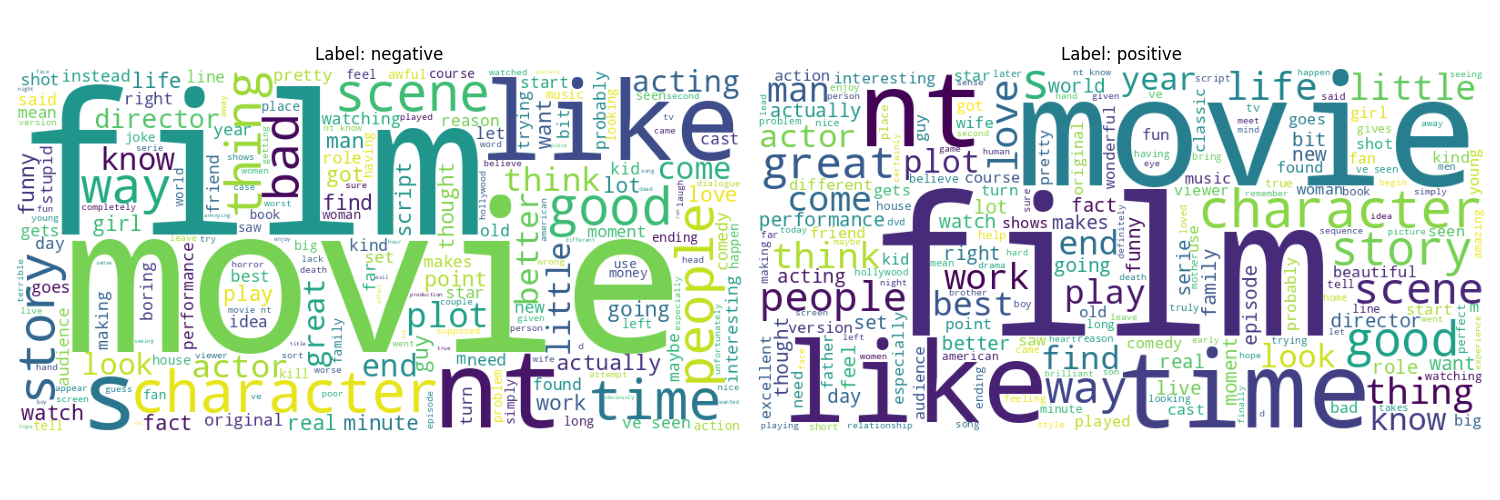
\includegraphics[width=0.8\textwidth]{raw_wordcloud.png}
    \caption{Word Cloud of Raw Preprocessed Reviews}
    \label{fig:raw_wordcloud}
\end{figure}

\begin{figure}[h]
    \centering
    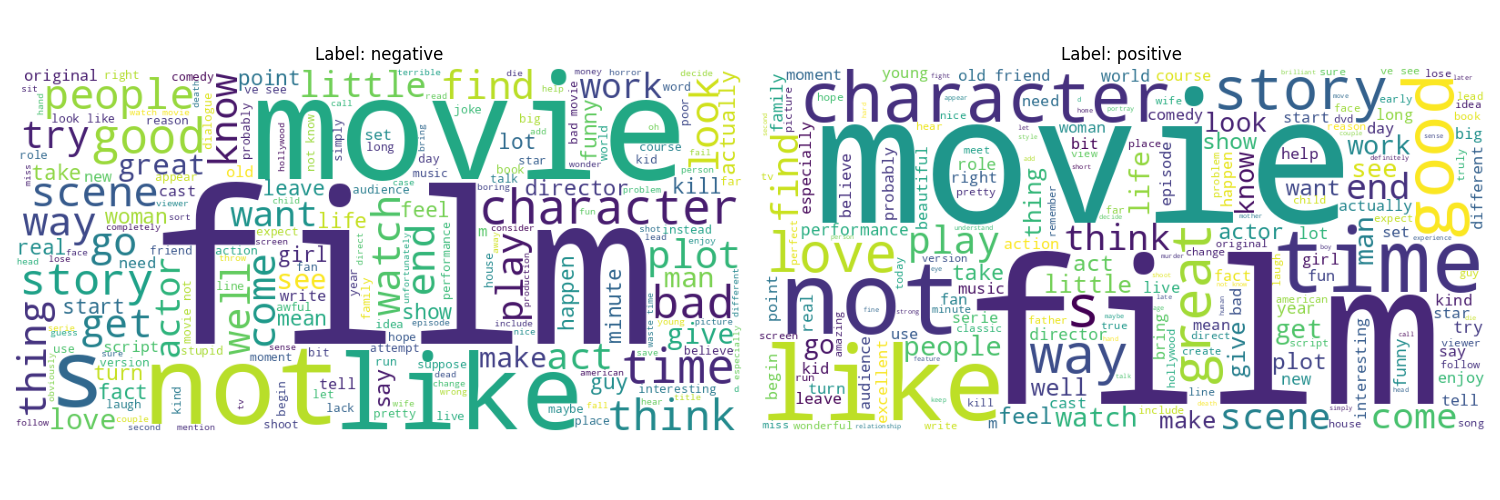
\includegraphics[width=0.8\textwidth]{lemma_wordcloud.png}
    \caption{Word Cloud of Lemmatized Reviews}
    \label{fig:lemma_wordcloud}
\end{figure}

Analysis of word frequencies reveals several interesting patterns:

\paragraph{General Observations}
\begin{itemize}
    \item \textbf{Domain-Specific Terms}: "movie" and "film" are consistently the most frequent words across both sentiment classes and preprocessing methods, indicating their role as domain identifiers rather than sentiment indicators.
    
    \item \textbf{Common Base Words}: Terms like "like", "time", "people", and "characters" appear frequently in both positive and negative reviews, suggesting they are neutral in sentiment.
\end{itemize}

\paragraph{Sentiment-Specific Patterns (after lemmatization)}
\begin{itemize}
    \item \textbf{Negative Reviews}:
        \begin{itemize}
            \item "bad" appears significantly more frequently (4,308 vs 2939 in positive reviews)
            \item Higher frequency of "not" (8,050 vs 5,419 in positive reviews)
            \item Focus on technical aspects: "plot", "acting", "scene"
        \end{itemize}
    
    \item \textbf{Positive Reviews}:
        \begin{itemize}
            \item Distinctive positive terms: "great" (2,775), "love" (2,259)
            \item "good" appears more frequently (4,347 vs 3,500 in negative reviews)
            \item More emphasis on emotional terms: "love", "great", "best"
        \end{itemize}
\end{itemize}

\paragraph{Impact of Lemmatization}
The lemmatization process had several notable effects:
\begin{itemize}
    \item \textbf{Word Consolidation}: 
        \begin{itemize}
            \item "movie" and "movies" were consolidated, increasing the frequency from 9,493 to 11,188 in negative reviews
            \item "character" and "characters" were combined
            \item "watch", "watching", and "watched" were merged into "watch"
        \end{itemize}
    
    \item \textbf{Negation Handling}: The contraction "nt" was properly transformed to "not", making it more prominent in the frequency counts
    
    \item \textbf{Verb Forms}: Various forms of verbs were consolidated (e.g., "see"/"seen", "act"/"acting"), providing clearer frequency patterns
\end{itemize}

These findings suggest that while some words are strong indicators of sentiment ("bad", "great", "love"), many frequent terms are neutral and context-dependent. The lemmatization process helped clarify word usage patterns by consolidating different forms of the same word, potentially improving the accuracy of subsequent sentiment analysis steps.
% -------------------------------------------------------------------------------------------------
% -------------------------------------------------------------------------------------------------
% -------------------------------------------------------------------------------------------------



\section{Vectorization}
Objective: Describe the vectorization technique used


% -------------------------------------------------------------------------------------------------
% -------------------------------------------------------------------------------------------------
% -------------------------------------------------------------------------------------------------



\section{Machine Learning Models}
Objective: Describe the machine learning model used and any specific training details.


% -------------------------------------------------------------------------------------------------
% -------------------------------------------------------------------------------------------------
% -------------------------------------------------------------------------------------------------



\section{Performance Metrics}
Objective: Present performance metrics (accuracy, precision, recall, F1 score) with interpretation of results.



% -------------------------------------------------------------------------------------------------
% -------------------------------------------------------------------------------------------------
% -------------------------------------------------------------------------------------------------



\section{Conclusions}
Objective: Summarize the results and discuss any notable observations across classes or preprocessing versions.



% -------------------------------------------------------------------------------------------------
% -------------------------------------------------------------------------------------------------
% -------------------------------------------------------------------------------------------------


\end{document}